\documentclass{article}

\usepackage{tikz}
\usetikzlibrary{calc}

\def\itempadding{1.5pt}

\def\drawbin#1{%
  \draw [#1] ($(0,0)+(-\itempadding,-\itempadding)$) 
  rectangle 
  ($(1,1)+(\itempadding,\itempadding)$);
}

\def\drawitem#1#2#3#4#5{%
  \draw [#3] 
  ($(0,#1)+(\itempadding,\itempadding)$) 
  rectangle node [#5] {#4} 
  ($(1,#2)+(-\itempadding,-\itempadding)$);
}

\begin{document}

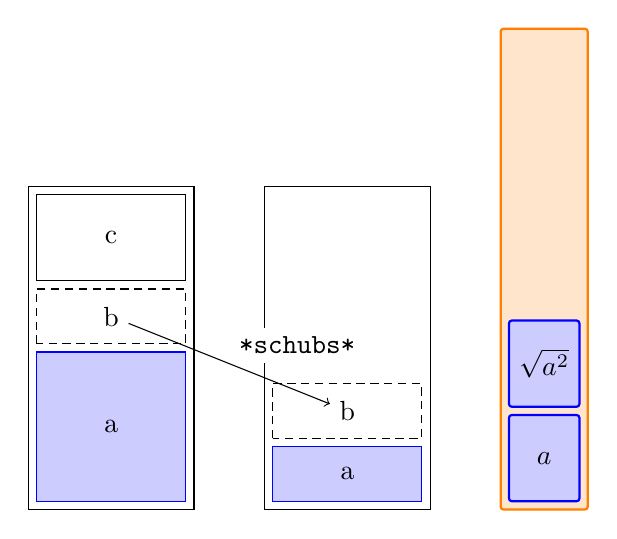
\begin{tikzpicture}
  
  \begin{scope}[x = 2cm, y = 4cm]
    \drawbin{}
    \drawitem{0}{.5}{fill = blue!20, draw=blue}{a}{}
    \drawitem{.5}{.7}{densely dashed}{b}{name = foo_before}
    \drawitem{.7}{1}{}{c}{}
  \end{scope}

  \begin{scope}[x = 2cm, y = 4cm, xshift = 3cm]
    \drawbin{}
    \drawitem{0}{.2}{fill = blue!20, draw=blue}{a}{}
    \drawitem{.2}{.4}{densely dashed}{b}{name = foo_after}
  \end{scope}

  \draw [->] (foo_before) to node [auto, fill=white] {\tt *schubs*} (foo_after);

  \begin{scope}[x = 1cm, y = 6cm, xshift = 6cm, rounded corners=1pt, thick]
    \drawbin{color = orange, fill = orange!20}
    \drawitem{0}{.2}{fill = blue!20, draw=blue}{$a$}{}
    \drawitem{.2}{.4}{fill = blue!20, draw=blue}{$\sqrt{a^2}$}{}
  \end{scope}

\end{tikzpicture}

\end{document}
